本章では ArchHDL での論理シミュレーションの実行時間を評価し,Icarus Verilog, NC-Verilog, VCS での論理シミュレーションの実行時間と比較する.

\begin{table}[t]
 \caption{実行環境}
 \label{table:exec_env}
 \begin{center}
  \begin{tabular}{l|c|c} \hline
         &  Icarus Verilog, ArchHDL  &  NC-Verilog, VCS   \\ \hline
  OS     &  Ubuntu12.04             &  CentOS5.9        \\
  CPU    &  Core i7-3770K 3.50GHz   &  Core i7-3770K 3.50GHz  \\
  メモリ  &  $16\,\mathrm{GB}$       &  $16\,\mathrm{GB}$  \\ \hline
  \end{tabular}
 \end{center}
\end{table}

\tabref{table:exec_env} に実行環境をまとめる.
評価には同じ仕様の 2 台の計算機を用いる.
一台は Icarus Verilog, ArchHDL の評価に用いる.もう一台は NC-Verilog, VCS の評価に用いる.
CPU,メモリなどのハードウェアの仕様は同一であるがソフトウェアの制約により異なる OS を利用する.

異なる OS を用いる理由を述べる.
NC-Verilog と VCS は RedHat 系のディストリビューションのみをサポートしている.
今回は RedHat 系のディストリビューションである CentOS5.9 を用いる.
しかし CentOS5.9 に含まれる gcc のバージョンは 4.1.2 である.
\ref{ss:modeling}節で述べたように,ArchHDL では C++11 のラムダ関数を用いて記述するため gcc のバージョンは 4.5 以上が必要である.
その条件を満たす Ubuntu12.04 を評価に用いる.
Ubuntu12.04 に含まれる gcc のバージョンは 4.6.3 である.
gcc の最適化オプションとして \verb/-O2/ を用いる.
Icarus Verilog はどちらのディストリビューションでも動作するが,今回は Ubuntu12.04 を用いる.
Ubuntu12.04 に含まれる Icarus Verilog のバージョンは 0.9.5 である.
VCS のバージョンは vcsC-2009.06 を用いる.NC-Verilog のバージョンは 06.20-s004 を用いる.

今回用いる計算機の CPU の物理コアは 4 コアであるため,OpenMP による並列化はスレッド数を 8 個にして評価する.

評価では,2 つのマイクロベンチマークと,現実的なハードウェアのベンチマークとしてステンシル計算回路\cite{koba:stencil}を用いる.
Verilog HDL と ArchHDL のためのハードウェアシミュレーションは手作業により作成した.
両ハードウェアシミュレーションの出力は同様になるように作成した.

評価結果に用いているラベルの名前について述べる.
オリジナルの ArchHDL は \textbf{ArchHDL} と表す.
\ref{sss:no_set} 節で述べた条件分岐の除去を適用したものを \textbf{NO SET} と表す.
\ref{sss:mem_copy} 節で述べたメモリ配置の工夫を適用したものを \textbf{MEM MAP} と表す.
\ref{ss:parallel} 節で述べた並列化を行ったものを \textbf{PARA} と表す.
メモリ配置の工夫と並列を同時に適用したものを \textbf{MEM MAP + PARA} と表す.


\subsection{マイクロベンチマークによる評価}

マイクロベンチマークとしてカウンタ回路と XORSHIFT による乱数生成回路を用いる.

\begin{figure}[t]
 \lstinputlisting[language=c++]{src/xorshift_alg.cc}
 \caption{XORSHIFT 法に基づく乱数生成のアルゴリズム}
 \label{src:xorshift_alg}
\end{figure}

カウンタ回路とは \figref{src:counter} に示した 1 サイクルごとに 1 を足す回路である.
ハードウェアの規模を増やすためにカウンタの数を指定できるようにした.
XORSHIFT による乱数生成回路とはシフトと XOR 演算のみで構成できる XORSHIFT 法に基づく乱数生成器をハードウェア記述によって実装した回路である.
\figref{src:xorshift_alg} に XORSHIFT 法に基づく乱数生成のアルゴリズムを C 言語によって実装したものを示す.

\begin{figure}[t]
 \centering
 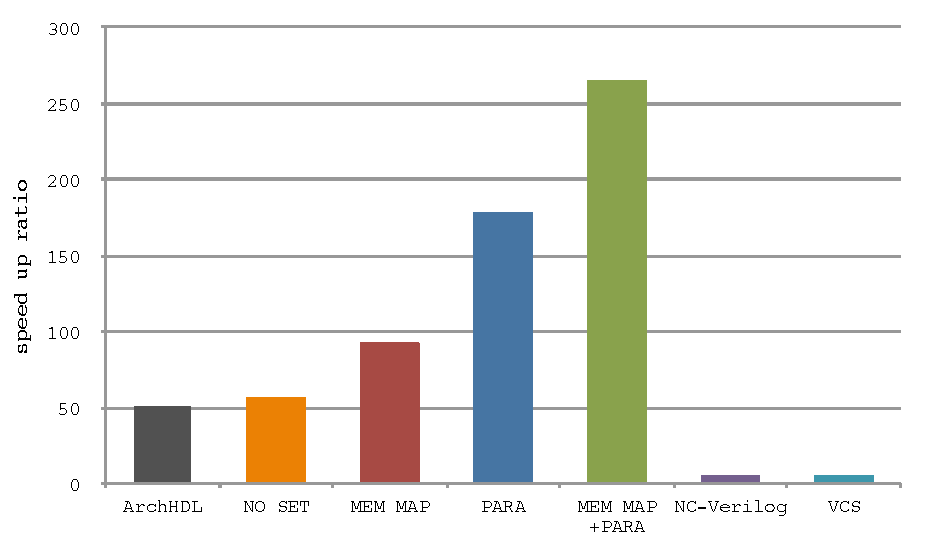
\includegraphics[clip,width=\linewidth]{counter_4096}
 \caption{4096 個のカウンタ回路の実行時間を Icarus Verilog と比較した速度向上比}
 \label{fig:counter4096}
\end{figure}

\figref{fig:counter4096} に 4096 個のカウンタ回路の実行時間を Icarus Verilog と比較した速度向上比を示す.
縦軸は Icarus Verilog での実行時間を 1 とした速度向上比を示している.

ArchHDL は商用の NC-Verilog, VCS と比較してもかなり高速である.
\textbf{MEM MAP + PARA} の論理シミュレーション実行時間は NC-Verilog の 58.8 倍,VCS の 56.7 倍高速である.

また今回提案している高速化手法はオリジナルの ArchHDL に比べていずれも効果が出ている.
\textbf{MEM MAP + PARA} の論理シミュレーション実行時間はオリジナルの ArchHDL の 5.23 倍高速である.



\begin{figure}[t]
 \centering
 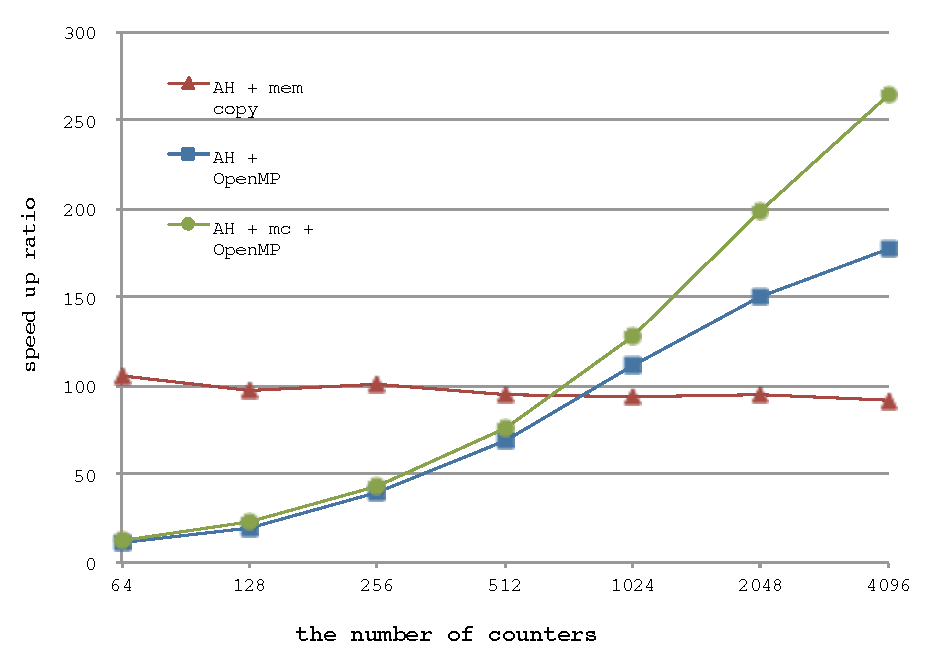
\includegraphics[clip,width=\linewidth]{counter_con}
 \caption{高速化手法を適用した ArchHDL と OpenMP を適用したカウンタ回路の実行時間を Icarus Verilog と比較した速度向上比}
 \label{fig:counter_con}
\end{figure}

\figref{fig:counter_con} に高速化手法を適用した ArchHDL と OpenMP を適用したカウンタ回路の実行時間を Icarus Verilog と比較した速度向上比を示す.
縦軸は Icarus Verilog での実行時間を 1 とした速度向上比を示している.
横軸はカウンタの個数である.

\textbf{MEM MAP} は逐次に実行されているので Icarus Verilog と比較した速度向上比はカウンタの個数を変えてもほとんど変わらない.
並列化を行った \textbf{PARA} と \textbf{MEM MAP + PARA} はカウンタの個数が 1024 個以上で \textbf{MEM MAP} よりも高速になる.
\textbf{PARA} より \textbf{MEM MAP + PARA} の方が常に高速であるので今回提案している逐次処理での高速化手法は並列化を行った場合でも効果が出ている.
カウンタの個数はハードウェアの規模とみなせるため,並列化が有効なのはある程度規模の大きい回路であると言える.


\begin{figure}[t]
 \centering
 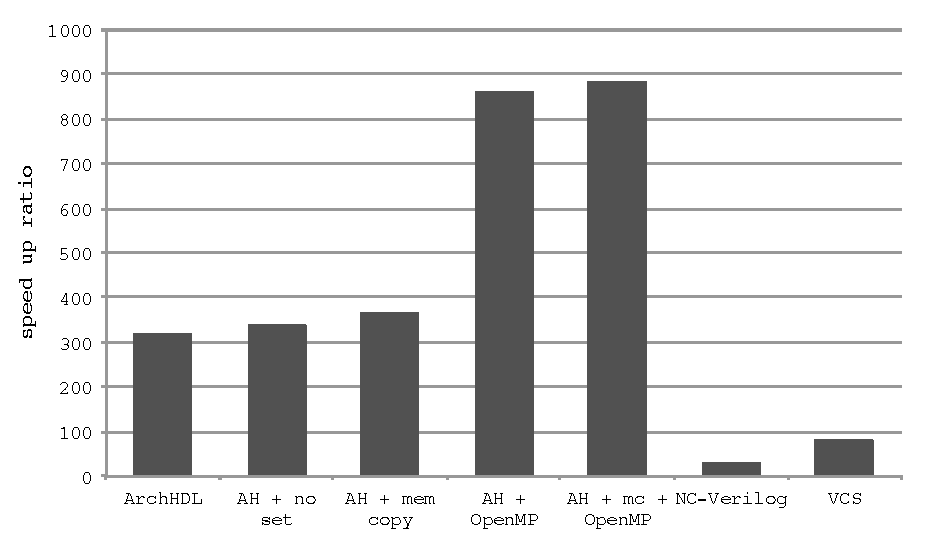
\includegraphics[clip,width=\linewidth]{xorshift}
 \caption{512 個の XORSHIFT による乱数生成器の実行時間を Icarus Verilog と比較した速度向上比}
 \label{fig:xorshift}
\end{figure}

\figref{fig:xorshift} は XORSHIFT による乱数生成器での実行時間を Icarus Verilog と比較した速度向上比である.
試行回数は 524,288 回である.初期値の異なる乱数生成器を 512 個用意している.

ArchHDL は商用の NC-Verilog, VCS と比較してもかなり高速である.
\textbf{MEM MAP + PARA} の論理シミュレーション実行時間は NC-Verilog の 32.2 倍,VCS の 11.3 倍高速である.

また今回提案している高速化手法はオリジナルの ArchHDL に比べていずれも効果が出ている.
\textbf{MEM MAP + PARA} の論理シミュレーション実行時間はオリジナルの ArchHDL の 2.78 倍高速である.


\subsection{ステンシル計算回路による評価}

\if0

\begin{table}[t]
 \caption{ステンシル計算回路でのプロファイリング結果 1.1}
 \label{table:stencil_prof1.1}
 \begin{center}
  % \setlength{\tabcolsep}{3pt}
  \begin{tabular}{lr} \toprule
  関数名 & 実行時間に占める割合 (\%) \\ \midrule
  reg::Update() (合計) & 16.57 \\
  ArchHDL::Step() & 12.47 \\
  brk & 15.05 \\ \bottomrule
  \end{tabular}
 \end{center}
\end{table}

\fi

\begin{figure}[t]
 \centering
 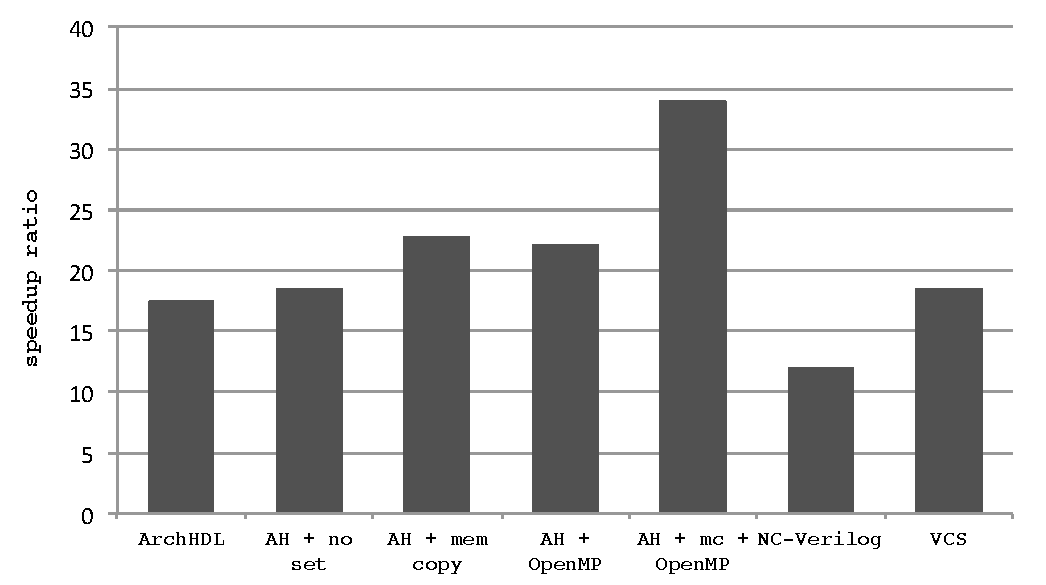
\includegraphics[clip,width=\linewidth]{stencil}
 \caption{ステンシル計算回路の Icarus Verilog と比較した実行時間の速度向上比}
 \label{fig:stencil}
\end{figure}

\figref{fig:stencil} はステンシル計算回路での実行結果である.
縦軸は Icarus Verilog と比較したそれぞれの速度向上比である.

オリジナルの ArchHDL は商用の NC-Verilog より高速であったが,同じく商用の VCS はオリジナルの ArchHDL と \textbf{NO SET} より高速である.
しかし逐次実行での高速化手法と並列化を共に適用した \textbf{MEM MAP + PARA} の論理シミュレーション実行時間は VCS の 1.83 倍高速である.

ステンシル計算回路の場合は Update() は 325,469,175 回呼ばれているのに対して,
reg の値に更新がないのは 5,145,760 回である.
つまり更新がないのは Update() メソッド呼び出し全体の $1.58\%$ 程度に過ぎない.
それにより条件分岐を無くす \textbf{NO SET} の論理シミュレーションはオリジナルの ArchHDL より高速である.
また Update() のメソッド呼び出しを減らし,かつメモリ配置を工夫している \textbf{MEM MAP} の論理シミュレーション実行時間はオリジナルの ArchHDL の 1.31 倍高速である.

また Module が 133 個,reg が 991 個存在する回路なので並列化の効果も大きい.
逐次実行での高速化手法と並列化を共に適用した \textbf{MEM MAP + PARA} の論理シミュレーション実行時間はオリジナルの ArchHDL の 1.95 倍高速である.


% \subsection{高速化の解析}
